% ================================== HEADER ====================================
\documentclass{article}           % Sets style/look of many things.
% \documentclass{report}          % part, chapters, front page etc.
\usepackage{exsheets}
\usepackage[utf8]{inputenc}       % Encoding of input files UTF-8
\usepackage[T1]{fontenc}
\usepackage[scaled]{beramono}     % Font
\usepackage{color}                % Color text
\usepackage{titlesec}             % Select alternative section titles
\usepackage{fancyvrb}
\usepackage{verbatim}             % Comment environment
\usepackage{listings}             % Format and render text/code etc.
\usepackage{minted}               % Much better syntax highlighting
\usepackage{float}                % Control of floating environment/figure
\usepackage{graphicx,  subfigure} % Better figures, graphics, units etc.
\usepackage{multicol}             % Multiple columns
\usepackage{amsmath}              % Math: Equation, split, align etc.
\usepackage{siunitx}              % SI units
\usepackage{mathtools}            % Different math tools to use with amsmath
\usepackage{amssymb}              % Math symbols
\usepackage[
    colorlinks,
    citecolor=black,              % I like links with standard black color
    filecolor=black,
    linkcolor=black,
    urlcolor=black
]{hyperref}                       % Links in TOC etc.
\usepackage[all]{hypcap}          % Better links to floating environment

\usepackage{tabto}
\newcommand\marginsymbol[1][0pt]{%
  \tabto*{0cm}\makebox[\dimexpr-1cm-#1\relax][r]{$\mathbb{P}$}\tabto*{\TabPrevPos}}

\renewcommand{\thesubsection}{\thesection.\alph{subsection}}
\title{\vspace{-2cm}INF3490/INF4490 Exercises Solutions - Week 3}
\author{Ole Herman S. Elgesem}
\date{\today}

% Removing paragraph indents is sometimes useful:
\setlength\parindent{0pt}

% Make margins smaller to fit more figures, tables etc on page: (optional)
\addtolength{\oddsidemargin}{-1.0in}
\addtolength{\evensidemargin}{-1.0in}
\addtolength{\textwidth}{2.0in}
\addtolength{\topmargin}{-0.8in}
\addtolength{\textheight}{1.6in}
% ==============================================================================

% ================================= DOCUMENT ===================================
\begin{document}
    \renewcommand\marginsymbol[1][0pt]{%
  \tabto*{0cm}\makebox[-1cm][c]{$\mathbb{P}$}\tabto*{\TabPrevPos}}

\maketitle
\(\mathbb{P}\) marks the programming exercises, we strongly recommend using
the python programming language for these. Exercises may be added/changed
after publishing.


\section{Pareto Optimality}
\begin{figure}[H]
  \centering
  \begin{minipage}[b]{0.45\textwidth}
    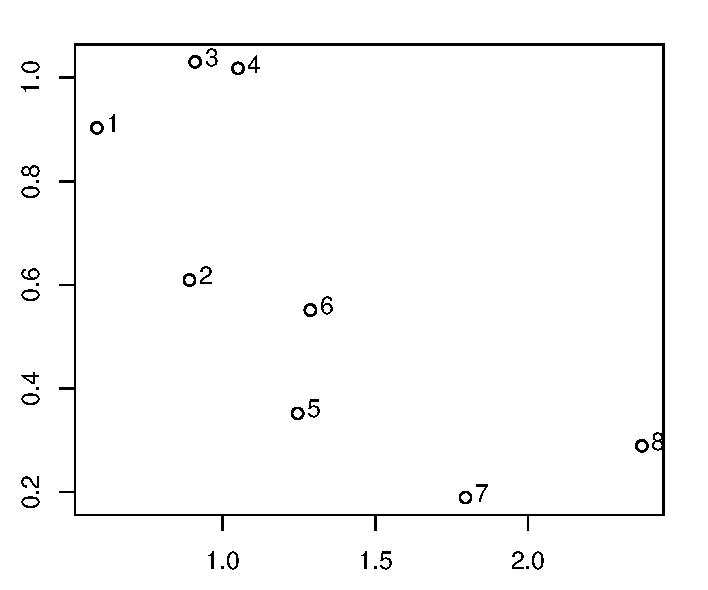
\includegraphics[width=\textwidth]{front_points_1.pdf}
    \caption{a}
  \end{minipage}
  \hfill
  \begin{minipage}[b]{0.45\textwidth}
    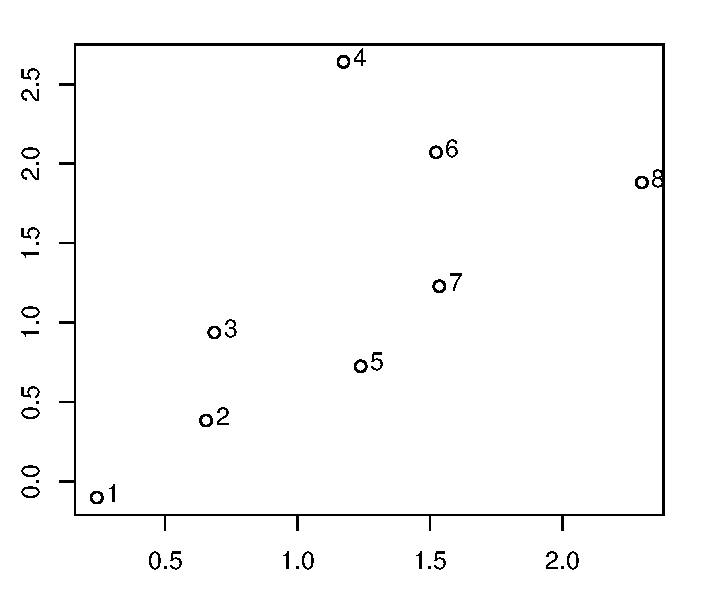
\includegraphics[width=\textwidth]{front_points_2.pdf}
    \caption{b}
  \end{minipage}
\end{figure}

For figure a and b above, find the Pareto optimal set when
\begin{itemize}
    \item Minimizing both \(f_1\) and \(f_2\)
    \item Minimizing \(f_1\), maximizing \(f_2\)
    \item Maximizing \(f_1\), minimizing \(f_2\)
    \item Maximizing both \(f_1\) and \(f_2\)
\end{itemize}

\emph{Answer:}\\
\begin{table}[H]
\centering
  \begin{tabular}{|c|c|c|}
    \hline
                             & a           & b             \\ \hline
    min \(f_1\), min \(f_2\) & \{1,2,5,7\} & \{1\}         \\ \hline
    min \(f_1\), max \(f_2\) & \{1,3\}     & \{1,2,3,4\}   \\ \hline
    max \(f_1\), min \(f_2\) & \{7,8\}     & \{1,2,5,7,8\} \\ \hline
    max \(f_1\), max \(f_2\) & \{3,4,6,8\} & \{4,6,8\}     \\ \hline
  \end{tabular}
  \caption{}
  \label{tab:task1}
\end{table}

\section{Weighted sum}
In figures a and b, what would be the maximum point when using weighted sum:
\begin{itemize}
    \item \(w_1 = 1\),  \(w_2 = 1\)
    \item \(w_1 = -1\), \(w_2 = 1\)
\end{itemize}
\emph{Answer:}\\
\begin{align*}
    w_1 &=  1 & w_2 &= 1 & \Rightarrow && \max a &= 8 & \max b &= 8\\
    w_1 &= -1 & w_2 &= 1 & \Rightarrow && \max a &= 1 & \max b &= 4
\end{align*}

\section{Hybrid Algorithm}
Why can hybrid algorithms make it harder to maintain diversity?\\

\emph{Answer:}\\

Hybrid initialization can lead to very uneven initial coverage of the search space, which might hamper the search.
Hybrid crossover and mutation, as well as (Lamarckian) local search before evaluation will lead solutions towards clusters near (local) optima.

\section{Measuring algorithm performance}
Why is it usually better to use the number of fitness function evaluations as a time measure,
rather than the number of generations, or the amount of CPU time spent?\\

\emph{Answer:}\\

Actual CPU time will change based on the resources available on the machine when running the algorithm.
This means that the hardware and running software (circumstances) will affect the measured time.
The evaluation is usually the most computationally intensive part of the algorithm, and is invariant across optimization algorithms since it is strictly problem dependent.
To improve performance we want to minimize the amount of evaluations,
and thus using it as a measurement makes sense.
Number of evaluations is only dependent on the algorithm, not on circumstances.
\section*{Contact and Github}
Corrections of grammar, language, notation or suggestions for improving this material are appreciated.
E-mail me at \href{mailto:olehelg@uio.no}{\textbf{olehelg@uio.no}} or use \href{https://github.com/olehermanse/INF3490-AI_Machine_Learning}{\textbf{GitHub}} to submit an issue or create a pull request.
The \href{https://github.com/olehermanse/INF3490-AI_Machine_Learning}{\textbf{GitHub repository}} contains all source code for assignments, exercises, solutions, examples etc.
As many people have been involved with writing and updating the course material, they are not all listed as authors here.
For a more complete list of authors and contributors see the \href{https://github.com/olehermanse/INF3490-AI_Machine_Learning/blob/master/README.md}{\textbf{README}}.

\end{document}
% ==============================================================================
